\section*{Problem 2 - Attitude Control using Euler Angles}
\subsection*{Problem 2.1}
The Lyapunov function candidate and the PD-controller can be written as 

\begin{equation}
\begin{aligned}\label{eq:yes}
	V &= \frac{1}{2} \boldsymbol{\omega}^{\top} \mathbf{I}_{CG} \boldsymbol{\omega} + \frac{1}{2} \tilde{\Theta}^{\top} \mathbf{K}_p \tilde{\Theta} \\
	\boldsymbol{\tau} &= -\mathbf{K}_d \boldsymbol{\omega} -\mathbf{T}_{\Theta}^{\top}(\Theta) \mathbf{K}_p \tilde{\Theta}
\end{aligned}
\end{equation}


Since $\boldsymbol{I}_{CG}$, $\boldsymbol{K}_d$ and $\boldsymbol{K}_p$ are symmetric, $\dot{V}$ becomes
\begin{equation} \label{eq:as}
\dot{V} = \boldsymbol{\omega}^T\boldsymbol{I}_{CG}\dot{\boldsymbol{\omega}} + \tilde{\Theta}^T\boldsymbol{K}_p\dot{\Theta}
\end{equation}

Inserting  (\ref{eq:kinetics}) into (\ref{eq:as})

\begin{equation}
\dot{V} = \boldsymbol{\omega}^T\left( \tau + (\boldsymbol{I}_{CG}\boldsymbol{\omega})\times \omega \right)
\end{equation}

\subsection*{Problem 2.2}
Answer Problem 2.2 here.

\subsection*{Problem 2.3}
Answer Problem 2.3 here.

\subsection*{Problem 2.4}
Answer Problem 2.4 here. Figures can be inserted as:
\begin{figure}[ht]
	\centering
	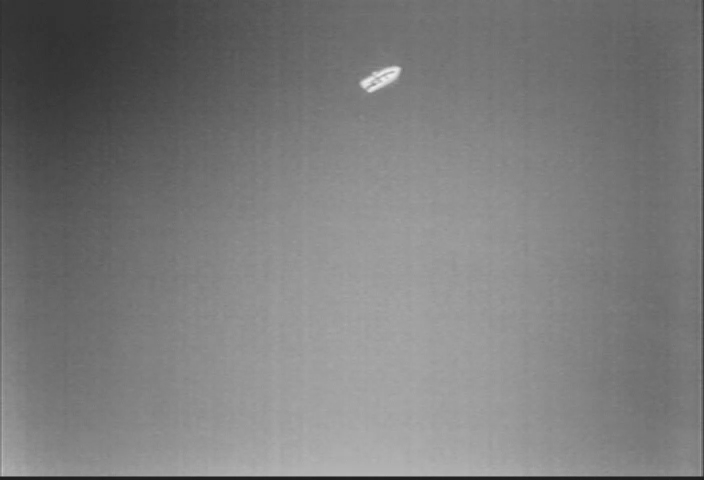
\includegraphics[width=0.7\textwidth]{fig1} % Filename is "fig1.png" and must be located in the same folder as this file. 
	\caption{Figure of something useful.}
	\label{fig:fig1}
\end{figure}

You can now refer to this figure as \figref{fig:fig1}. You can also insert figures side-by-side:
\begin{figure}[ht]
	\centering
	\begin{subfigure}[b]{0.45\textwidth}
		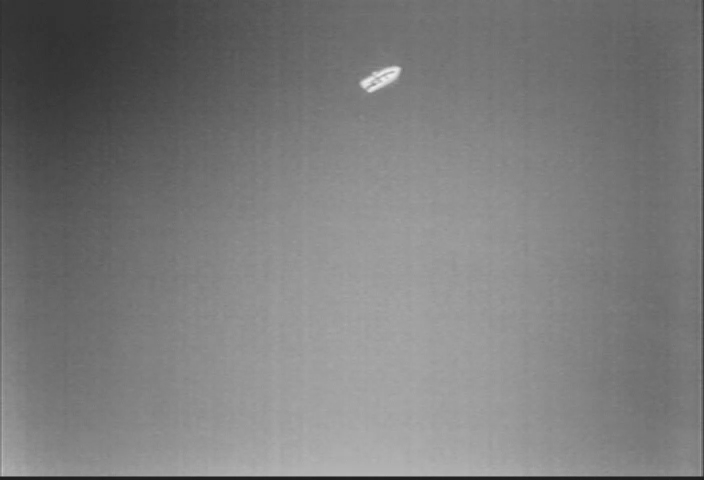
\includegraphics[width=\textwidth]{fig1}
		\caption{Fig 2a)}
		\label{fig:2a}
	\end{subfigure}
	~ %add desired spacing between images, e. g. ~, \quad, \qquad, \hfill etc. 
	%(or a blank line to force the subfigure onto a new line)
	\begin{subfigure}[b]{0.45\textwidth}
		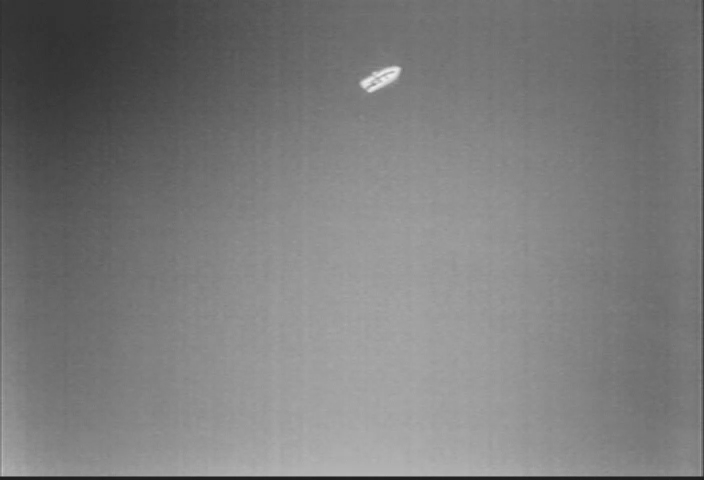
\includegraphics[width=\textwidth]{fig1}
		\caption{Fig 2b)}
		\label{fig:2b}
	\end{subfigure}
	\caption{Caption for both figures}\label{fig:2}
\end{figure}